\chapter{Imote2 Hardware}
For this thesis the Imote2~\cite{imote2} hardware platform was used as it allowed us to use
standard Linux environment while acting like a wireless sensor network node to
the outside. The Imote2 platform
consists of different pluggable boards to extend it with sensors or multimedia
capabilities. For our work we only used the Imote2 Processor Radio Board
(IPR2400) and the Interface Board (IIB2400) for serial console access and JTAG.

While other sensor nodes are tightly constrained regarding their computing power
and storage, the Imote2 is based on a powerful XScale CPU and equipped with 32
MByte of SDRAM as well as flash storage. This comes of course with a higher power
consumption cost compared to microcontroller based sensor nodes like the T-Mote
Sky~\footnote{http://www.snm.ethz.ch/Projects/TmoteSky}. On the other hand
exactly these components are allowing us to run a full
Linux and DTN system on the node and allow comfortable development and rapid
prototyping.

\section{Processor Radio Board}
As the name suggests this is the base board all other boards rely on. It holds
the PXA271 XScale ARM System on a Chip with a CPU frequency from 13 to 416 MHz
as well as the SDRAM and flash storage. If configured for a frequency from 13
to 104 MHz the CPU can be used in a low power mode on a low voltage level
(0.85V). This was not done during this work, but would be an interesting target
for later deployment. Instead we used the CPU at the full frequency of 416 MHz
during development and evaluation.

The PXA271 offers a wide range of peripheral components already built in. The
connectors for these are available on the basic and advanced connectors on the
board. Examples are USB host and client, SDIO, UART, AC97 and I2S audio
interfaces, I2C, SPI and GPIOs. USB client is already routed to a mini USB
connector on the board. This can be used to access the system and supply power
over USB.

Figure~\ref{fig:imote2top} is a top view of the IPR2400 showing the USB client plug,
the board connectors and the IEEE 802.15.4 radio transceiver with the onboard
antenna. We go into more details about it in section~\ref{cc2420}.

\begin{figure}
  \begin{center}
    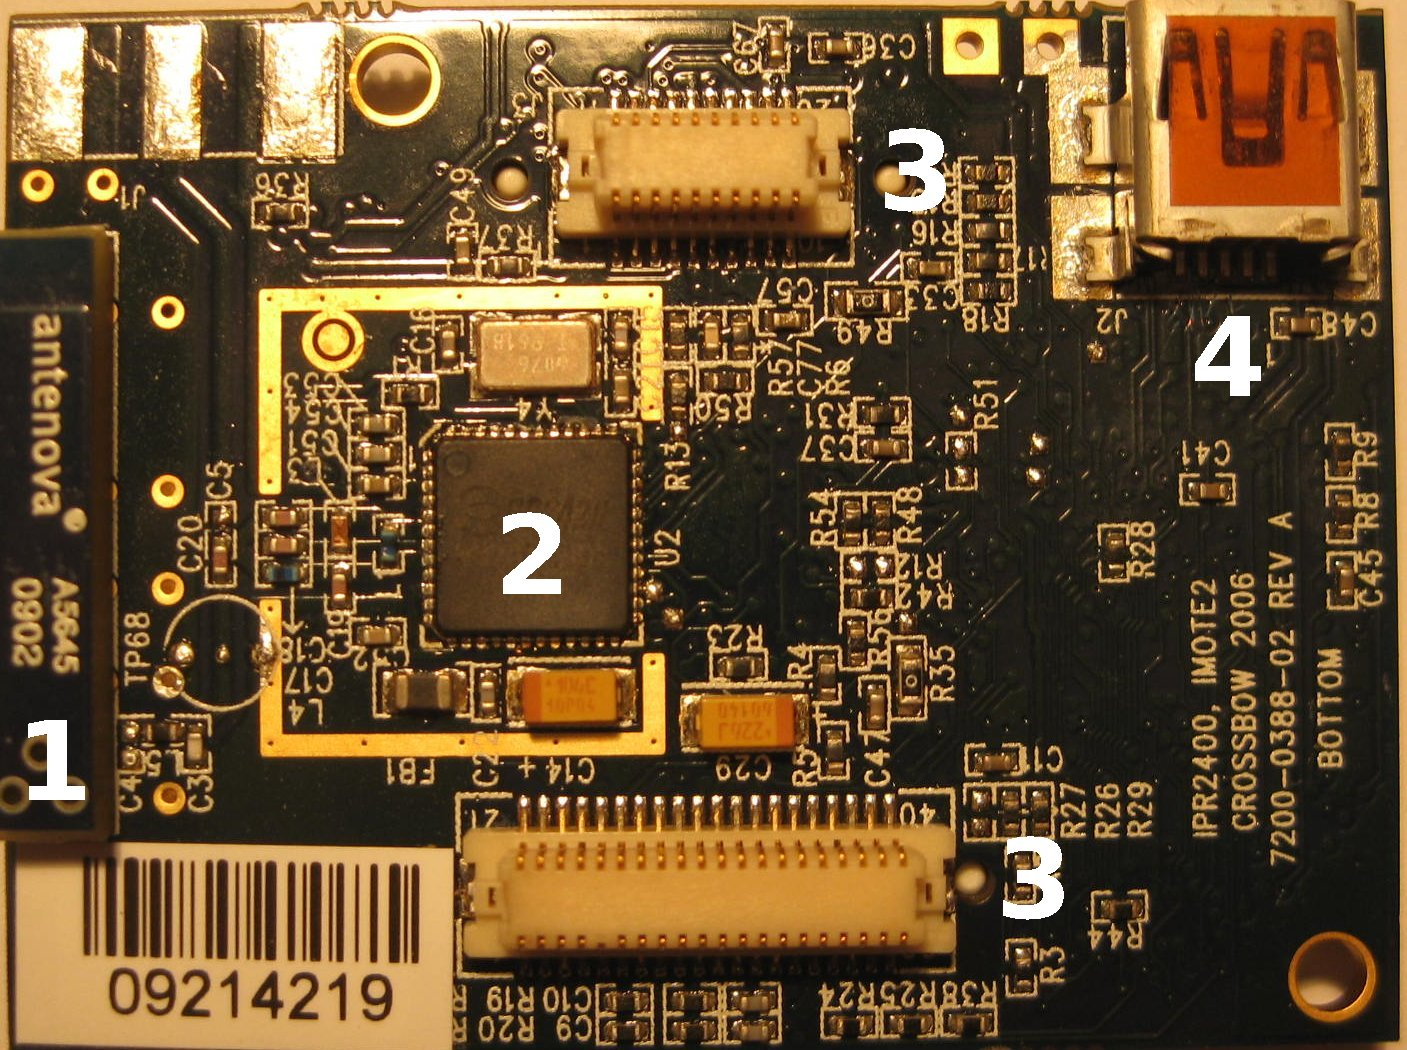
\includegraphics[width=6.5cm]{images/imote_top_cutted2}
    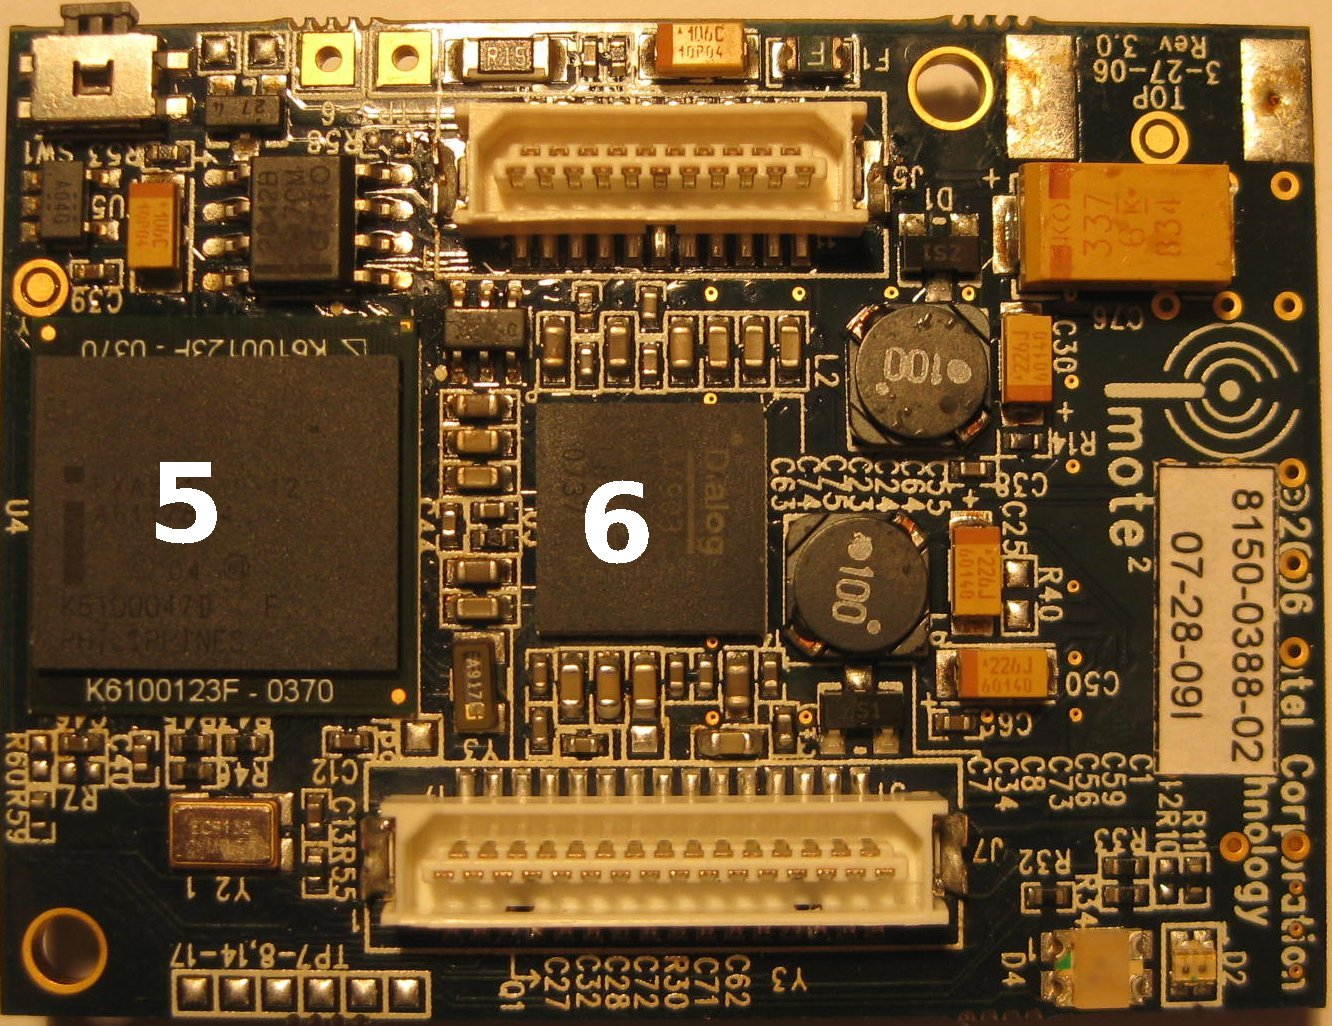
\includegraphics[width=6.5cm]{images/imote_bottom_cutted2}
    \caption{Top side of the Processor Radio Board with antenna (1), the CC2420 (2),
	     the board connectors (3) and the USB connector (4) on the left side
	     and the bottom side with the PXA processor (5) and power management
	     chip (6) on the right}
        \label{fig:imote2top}
  \end{center}
\end{figure}

\section{CC2420 IEEE 802.15.4 Transceiver}
\label{cc2420}
The IEEE 802.15.4 radio used on the Imote2 is a CC2420~\cite{cc2420} from TI (formerly ChipCon).
Configuration and data transfer is done over SPI while some extra signalling
GPIOs are used for interrupts. The hardware also features a FIFO for transmit as
well as for receive. Both FIFOs have a size of 128 bytes which is the maximum
transfer unit in IEEE 802.15.4. Interrupts are generated once a start frame delimiter
(SFD) has been recognized, a full packet has arrived in the FIFO or when a FIFO is
about to reach a specified threshold.

The CC2420 is a full-function device (FFD) and as such can be used as
coordinator or normal node. It uses only the 2.4 GHz band out of the three
available and supports all sixteen channels on this band (channel 11 / 2.405 GHz
to channel 26 / 2.480 GHz). It also supports the highest data rate available
in IEEE 802.15.4 with 250 kbps. Configuration modes for the radio transmission power
are available to either save power or extend range. The CC2420 falls in the
category of packet-based radio. Packet-based radios are implementing parts of
the physical layer already in hardware. This brings the benefit of less software
complexity to drive the chip.

Additional hardware support is available for CRC calculation, data encryption, clear
channel assignment, auto acknowledge, link quality indication and more. Due to
his extensive hardware support this chip is also used in many microcontroller
based systems. It is easy to integrate the SPI interface as well as the GPIO and
interrupt lines into a system and the software support to drive the chip can be
stripped down to a minimum if needed.

The only disadvantage is the lack of support for all frequency bands. The 2.4 GHz
industrial, scientific and medical (ISM) band is already crowded with WiFi
communication, baby monitors, home video streaming solutions and many other
transmitters. Having a chip that would be able to use the other radio bands
would have opened the possibility to switch to a less crowded band and evaluate
the performance in contrast to the 2.4 GHz band.
